\section{Desarrollo}
Esta actividad requiere comprender cómo funcionan los pines GPIO de la Raspberry Pi y su capacidad para interactuar con dispositivos electrónicos. Un servomotor es un dispositivo que permite el control preciso del ángulo de rotación, mientras que los LEDs y el buzzer proporcionan señales visuales y auditivas respectivamente. Mediante la programación, se controlará el movimiento del servomotor y la activación de los LEDs y el buzzer.

\subsection{Materiales necesarios}
Para esta práctica, se requieren los siguientes componentes:
\begin{itemize}
	\item \textbf{Raspberry Pi} (cualquier modelo con pines GPIO disponibles).
	\item \textbf{2 LEDs} (verde y rojo).
	\item \textbf{Resistencias de 220\textohm} (para limitar la corriente del LED y evitar daños).
	\item \textbf{Buzzer}.
	\item\textbf{Servomotor}
	\item \textbf{Cables de conexión}.
	\item \textbf{Protoboard} (para facilitar las conexiones).
\end{itemize}

\subsection{Conexión del circuito}
La conexión de los componentes se realizará de la siguiente manera:
\begin{itemize}
	\item El \textbf{cable de control} del servomotor se conecta a un \textbf{pin GPIO} de la Raspberry Pi. 
	\item El \textbf{ánodo (+) del LED} verde se conecta a un \textbf{pin GPIO} de la Raspberry Pi a través de la resistencia de 220\textohm, y el \textbf{cátodo (-)} a \textbf{GND}.
	\item El \textbf{ánodo (+) del LED} rojo se conecta a otro \textbf{pin GPIO} de la Raspberry Pi a través de la resistencia de 220\textohm, y el \textbf{cátodo (-)} a \textbf{GND}.
	\item El \textbf{pin positivo} del buzzer se conecta a un \textbf{pin GPIO}, y el pin negativo a \textbf{GND}.
\end{itemize}

\subsection{Explicación del funcionamiento}
\begin{enumerate}
	\item Se configura la Raspberry Pi para controlar el servomotor, el buzzer y los LEDs.
	\item Al recibir la señal de apertura, el servomotor rota hasta el ángulo especificado, el LED verde se enciende y el buzzer emite un sonido.
	\item Al recibir la señal de cierre, el servomotor regresa a su posición original y el LED rojo se enciende.
	\item Se utiliza un breve retraso en la programación para asegurar la correcta ejecución de las acciones.
\end{enumerate}

\subsection{Pruebas y resultados}
Para verificar el funcionamiento del sistema:
\begin{itemize}
	\item Conectar todos los componentes correctamente.
	\item Ejecutar el programa en la Raspberry Pi.
	\item Observar cómo el servomotor se mueve, el LED verde se enciende y el buzzer emite un sonido al abrir la puerta, y cómo el LED rojo se enciende al cerrar la puerta.
\end{itemize}

Si algún componente no responde correctamente, revisar la hoja de datos, así como, las conexiones y el código.

\subsection{Aplicaciones y mejoras}
Este sistema básico puede extenderse con diversas mejoras, como:
\begin{itemize}
	\item \textbf{Uso de sensor de proximidad} para automatizar la apertura y cierre del servomotor.
	\item \textbf{Conexión a una interfaz web}, integrando tecnologías como Flask o MQTT para manejar el LED desde otro dispositivo.
	\item \textbf{Integración de un sistema de seguridad} que registre los eventos de apertura y cierre.
\end{itemize}

\begin{figure}[h]
	\centering
   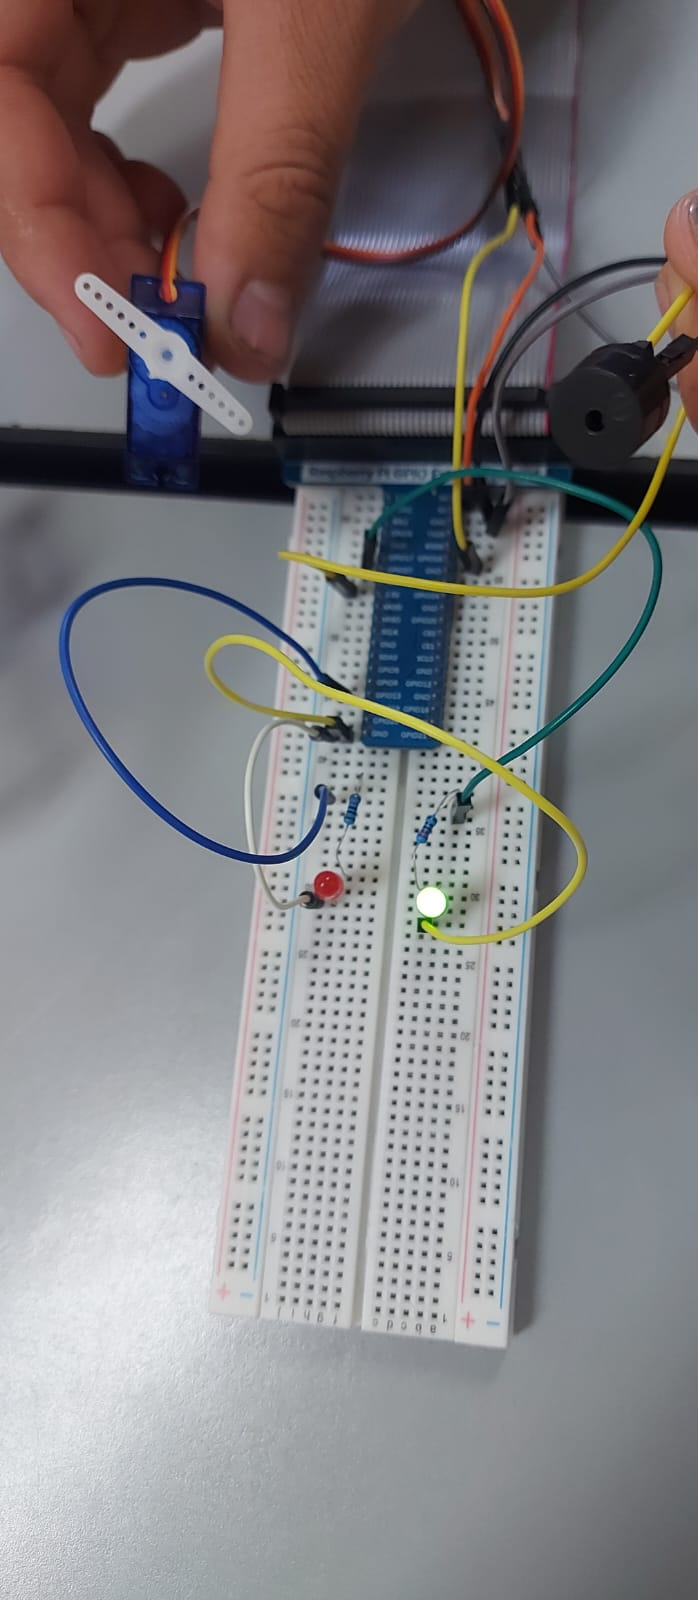
\includegraphics[width=0.5\textwidth]{imagenes/ledVerde_buzzer_servo.jpg} 
	\caption{Servomotor abierto, por ende, led verde encendido y buzzer sonando}
\end{figure}

\begin{figure}[h]
	\centering
	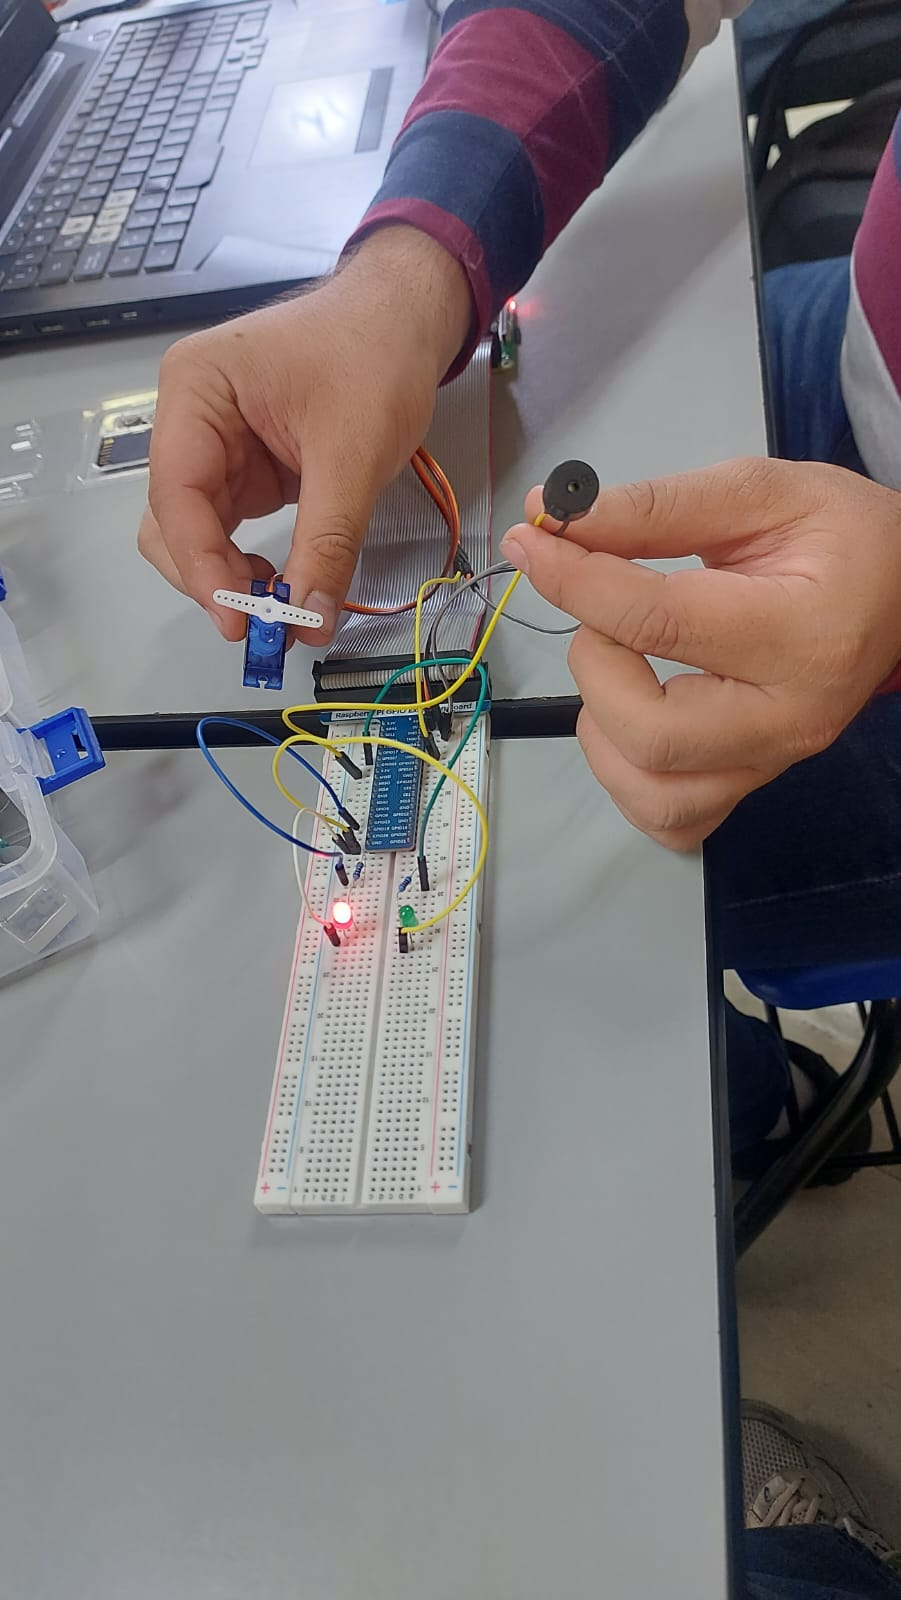
\includegraphics[width=0.5\textwidth]{imagenes/ledRojo_servo.jpg}
	\caption{Servomotor cerrado, por ende, led rojo encendido}
\end{figure}

\newpage